\section{Divide and conquer algorithms}

The divide and conquer design paradigm consists of three key steps:
\begin{enumerate}
    \item Divide the problem into smaller sub-problems. 
    \item Conquer the sub-problems by solving them recursively. 
    \item Combine the solutions of the sub-problems.
\end{enumerate}
This approach enables us to tackle larger problems by breaking them down into smaller, more manageable pieces, often resulting in faster overall solutions.

The divide step is typically constant, as it involves splitting an array into two equal parts. 
The time required for the conquer step depends on the specific algorithm being analyzed.
Similarly, the combine step can either be constant or require additional time, again depending on the algorithm.

\paragraph*{Merge sort}
The merge sort algorithm, previously discussed, follows these steps:
\begin{itemize}
    \item \textit{Divide}: the array is split into two sub-arrays.
    \item \textit{Conquer}: each of the two sub-arrays is sorted recursively.
    \item \textit{Combine}: the two sorted sub-arrays are merged in linear time.
\end{itemize}
The recursive expression for the complexity of merge sort can be expressed as follows:
\[T(n)=\underbrace{2}_{\#\text{subproblems}} \underbrace{T\left(\dfrac{n}{2}\right)}_{\text{subproblem size}}+\underbrace{\Theta(n)}_\text{work dividing and combining}\]

\subsection{Binary search}
The binary search problem involves locating an element within a sorted array. 
This can be efficiently solved using the divide and conquer approach, outlined as follows:
\begin{enumerate}
    \item \textit{Divide}: select half of the array to search for the element.
    \item \textit{Conquer}: check the middle element of the sub-array.
    \item \textit{Combine}: if the element is found, return its index in the array.
\end{enumerate}
In this scenario, we only have one sub-problem, which is the new sub-array, and its length is half that of the original array.
Both the divide and combine steps have a constant complexity.

Thus, the final expression for the complexity is:
\[T(n)=1T\left(\dfrac{n}{2}\right)+\Theta(1)\]

By applying the master method, we find a final complexity of:
\[T(n)=\Theta(\log n)\]

\subsection{Power of a number}
The problem at hand is to compute the value of $a^n$, where $n\in\mathbb{N}$. 
The naive approach involves multiplying $a$ by itself $n$ times, resulting in a total complexity of $\Theta(n)$. 

We can also use a divide and conquer algorithm to solve this problem by dividing the exponent by two, as follows:
\[a^n=\begin{cases} a^\frac{n}{2}\cdot a^\frac{n}{2}  \:\:\:\:\qquad\qquad \text{if }n\text{ is even} \\ a^\frac{n-1}{2}\cdot a^\frac{n-1}{2} \cdot a \qquad \text{if }n\text{ is odd} \end{cases}\]
In this approach, both the divide and combine phases have a constant complexity, as they involve a single division and a single multiplication, respectively. 
Each iteration reduces the problem size by half, and we solve one sub-problem (with two equal parts).

Thus, the recurrence relation for the complexity is:
\[T(n)=1T\left(\dfrac{n}{2}\right)+\Theta(1)\]
By applying the master method, we find a final complexity of:
\[\Theta(\log n)\]

\subsection{Matrix multiplication}
Matrix multiplication involves taking two matrices $A$ and $B$ as input and producing a resulting matrix $C$, which is their product.
Each element of the matrix $C$ is computed as follows:
\[c_{ij}=\sum_{k=1}^{n}a_{ik}\cdot b_{kj}\]
The standard algorithm for matrix multiplication is outlined below:
\begin{algorithm}[H]
    \caption{Standard matrix multiplication}
        \begin{algorithmic}[1]
            \For{$i = 1$ \textbf{to} $n$} 
                \For{$j = 1$ \textbf{to} $n$} 
                    \State $c_{ij} = 0$
                    \For{$k = 1$ \textbf{to} $n$} 
                        \State $c_{ij} = c_{ij}+a_{ik} b_{kj}$
                    \EndFor
                \EndFor
            \EndFor
        \end{algorithmic}
\end{algorithm}
The complexity of this algorithm, due to the three nested loops, is $\Theta(n^3)$.

\paragraph*{Divide and conquer}
For the divide and conquer approach, we divide the original $n\times n$ matrix into four $\frac{n}{2}\times\frac{n}{2}$ sumatrices: 
\[\begin{bmatrix} r & s \\ t & u \end{bmatrix}=\begin{bmatrix} a & b \\ c & d \end{bmatrix} \cdot \begin{bmatrix} e & f \\ g & h \end{bmatrix}\]
This requires solving the following system:
\[\begin{cases} r = ae + bg \\ s = af + bh \\ t = ce + dg \\ u = cf + dh \end{cases}\]
This results in a total of eight multiplications and four additions of the submatrices. 
The recursive part of the algorithm involves the matrix multiplications. 
The time complexity can be expressed as $T(n)=8T\left(\frac{n}{2}\right)+\Theta(n^2)$.
Using the master method, we find that the total complexity remains $\Theta(n^3)$.

\paragraph*{Strassen}
To improve efficiency, Strassen proposed a method that reduces the number of multiplications from eight to seven matrices.
This approach requires seven multiplications and a total of eighteen additions and subtractions.

The divide and conquer steps are as follows:
\begin{enumerate}
    \item \textit{Divide}: partition matrices $A$ and $B$ into $\frac{n}{2}\times\frac{n}{2}$ submatrices and formulate terms for multiplication using addition and subtraction.
    \item \textit{Conquer}: recursively perform seven multiplications of $\frac{n}{2}\times\frac{n}{2}$ submatrices.
    \item \textit{Combine}: construct matrix $C$ using additions and subtractions on the $\frac{n}{2}\times\frac{n}{2}$ sumbatrices. 
\end{enumerate}
The recurrence relation for the complexity is: $T(n)=7T\left(\frac{n}{2}\right)+\Theta(n^2)$
By solving this recurrence with the master method, we obtain a complexity of:
\[\Theta\left(n^{\log_27}\right)\approx \Theta\left(n^{2.81}\right)\]

Although $2.81$ may not seem significantly smaller than $3$, the impact of this reduction in the exponent is substantial in terms of running time.
In practice, Strassen's algorithm outperforms the standard algorithm for $n \geq 32$.

The best theoretical complexity achieved so far is $\Theta\left(n^{2.37}\right)$, although this remains of theoretical interest, as no practical algorithm currently achieves this efficiency.

\subsection{VLSI layout}
The problem involves embedding a complete binary tree with $n$ leaves into a grid while minimizing the area used.
\begin{figure}[H]
    \centering
    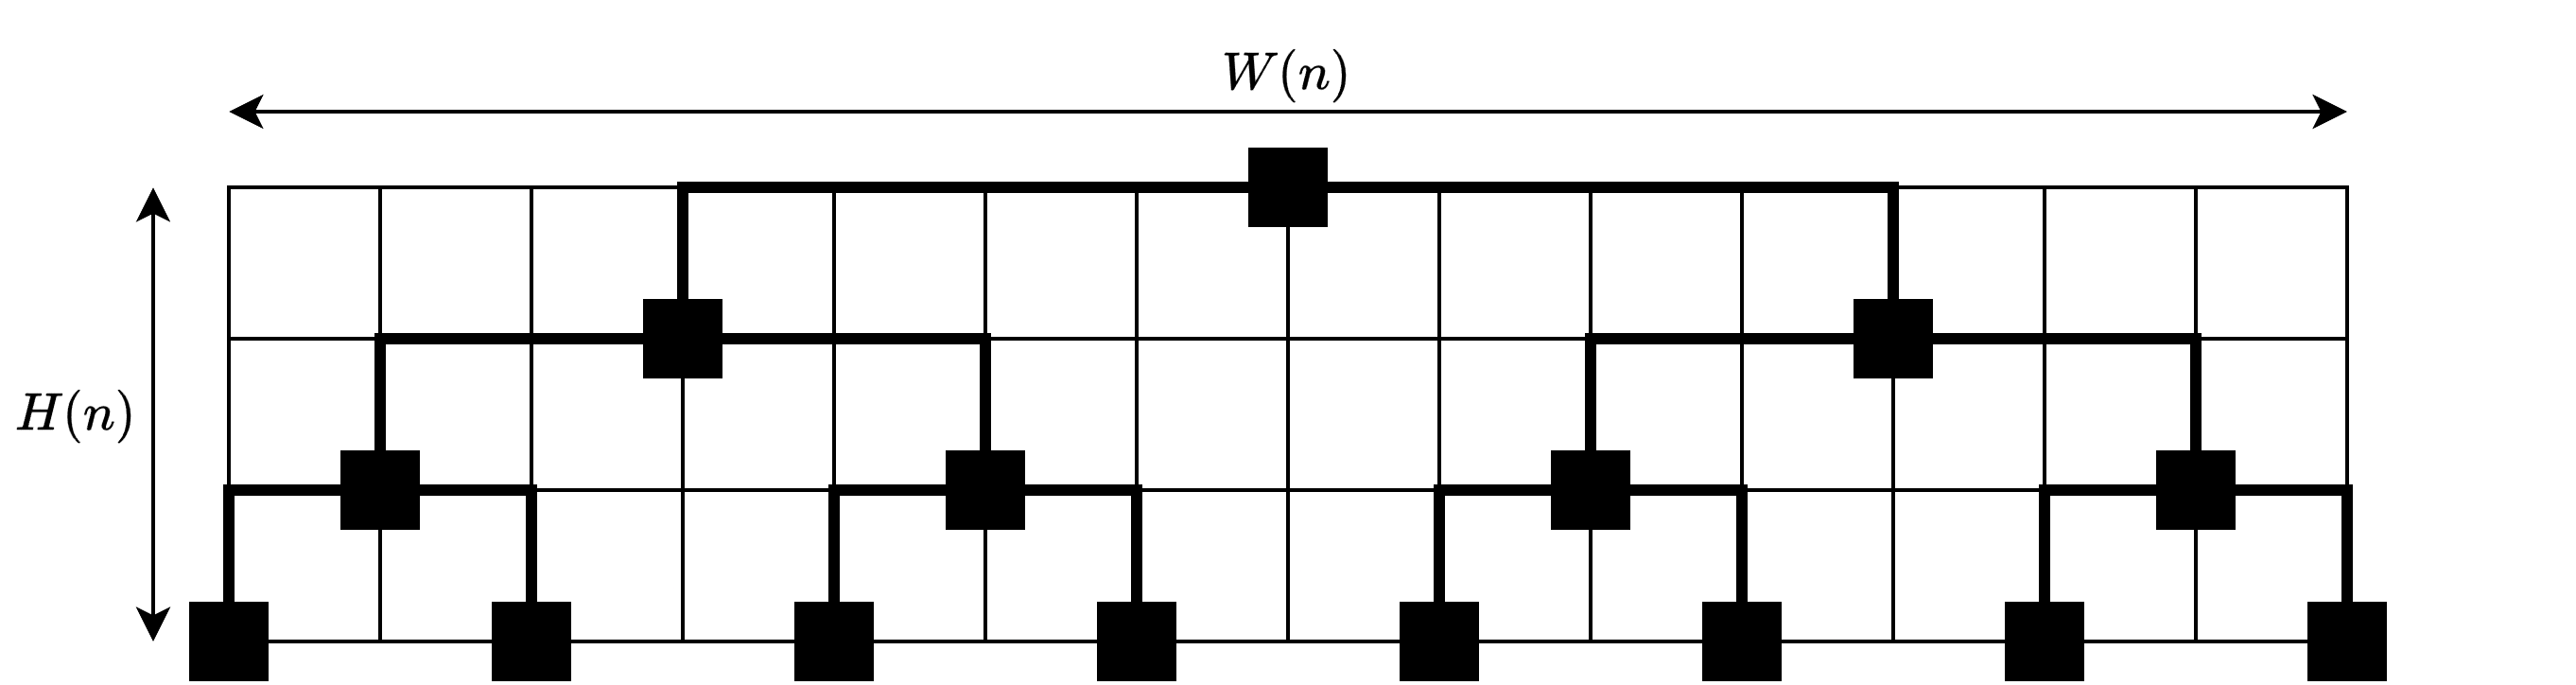
\includegraphics[width=0.9\linewidth]{images/vlsi.png}
    \caption{VLSI layout problem}
\end{figure}
For a complete binary tree, the height is given by:
\[H(n)=H\left(\dfrac{n}{2}\right)+\Theta(1)=\Theta(\log_2n)\]
The width is expressed as:
\[W(n)=2W\left(\dfrac{n}{2}\right)+\Theta(1)=\Theta(n)\]
Thus, the total area of the grid required is:
\[\text{Area}=H(n)\cdot W(n)=\Theta(n\log_2n)\]

\paragraph*{H-tree}
An alternative solution to this problem is to use an $h$-tree instead of a binary tree.
\begin{figure}[H]
    \centering
    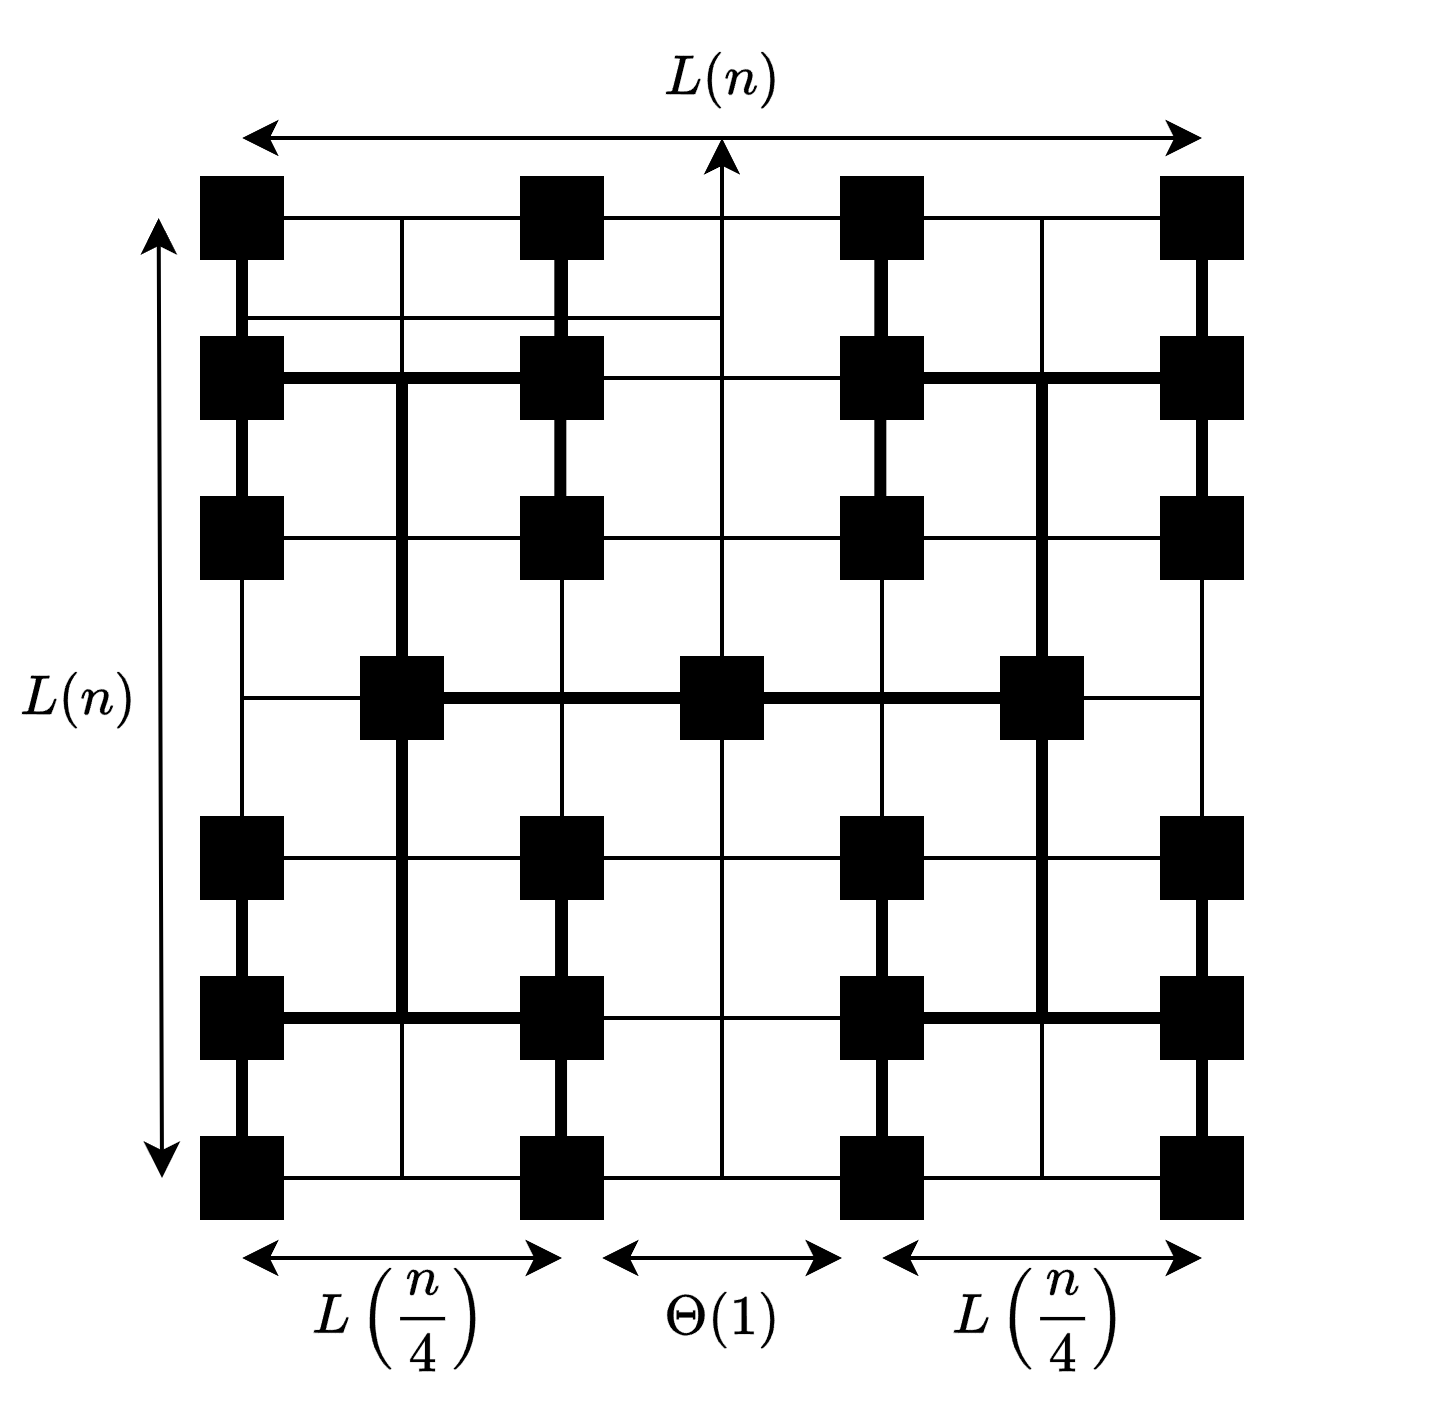
\includegraphics[width=0.55\linewidth]{images/vlsi1.png}
    \caption{VLSI layout problem}
\end{figure}
For the $h$-tree, the length is given by:
\[L(n)=2L\left(\dfrac{n}{4}\right)+\Theta(1)=\Theta(\sqrt{n})\]
Consequently, the total area required for the $h$-tree is computed as:
\[\text{Area}=L(n)^2=\Theta(n)\]